\documentclass[12pt, a4paper]{article}

\usepackage{mypreamble}
\usepackage{standalone}

\usepackage{tikz}

\usepackage{pdflscape}

\usepackage{biblatex}
\addbibresource{main.bib}

\title{Discrete Math II, HW I}
\date{March, 2023}
\author{Aminev Timur, M3104}


\newcommand\EGraph{\mathcal{G}^{*}}
\newcommand\EGraphL{\mathcal{G}}

\begin{document}
\maketitle

\problem The graph of Europe \(\EGraph = \Pair{V, E}\). Let \(\EGraphL\) be the
largest connected component of \(\EGraph\)

\begin{enumerate}[label=\alph*)]
\item \Cref{fig:map_basic} represents \(\EGraph\) with \textbf{no} intersecting
edges
\item \(|V| = 49\), \(|E| = 92\)

In order to count degree of each node, we should go through all edges, and
increment degree of a vertex if the edge contains the vertex.
The way it was calculated can be found
\href{https://github.com/ablearthy-itmo-39828cf299f04949c86/discrete-math-2-hw-1/blob/c665370/auto/general.py}{here}
\begin{align*}
\delta(\EGraphL) &= 1 \\
\Delta(\EGraphL) &= 9
\end{align*}

Radius, diameter and center can be obtained by calculating eccentricity for
each vertex (using BFS)

\begin{align*}
\rad(\EGraphL) &= 5 \\
\diam(\EGraphL) &= 8 \\
\mycenter(\EGraphL) &= \{\texttt{RUS}, \texttt{BLR}, \texttt{LTU}, \texttt{POL}, \texttt{UKR}, \texttt{CZE}, \texttt{DEU}, \texttt{SVK}, \texttt{HUN}, \texttt{HRV}, \texttt{AUT}, \texttt{CHE}, \texttt{SVN}\}
\end{align*}

\texttt{Girth} equals 3 --- \(\{\texttt{CHE}, \texttt{AUT}, \texttt{LIE}\}\)

Vertex and edges connectivity are obtained from the following observation:
\texttt{DNK} is connected only with \texttt{DEU}, therefore
\[\varkappa(\EGraphL) = \lambda(\EGraphL) = 1\]

\item \textbf{Minimum vertex coloring}. Due to \textit{four color theorem},
there're at most 4 colors needed. Let's explore is it possible to use less
colors? Let's try to use 3 colors. However, it's impossible to color countries
\texttt{HRV}, \texttt{SRB}, \texttt{BIH}, \texttt{MNE}. They're all connected
with each other, so three colors is not enough, therefore we have to use four
colors. I used SMT solver (Z3) to find function \(V \to \mathbb{N}\). Here's
\href{https://github.com/ablearthy-itmo-39828cf299f04949c86/discrete-math-2-hw-1/blob/753891b/auto/vertex_coloring.py}{the
script}. See \cref{fig:vertex_coloring_map}.

\item \textbf{Minimum edge coloring}. I used SMT solver (Z3). Here's
\href{https://github.com/ablearthy-itmo-39828cf299f04949c86/discrete-math-2-hw-1/blob/8bc76f0/auto/edge_coloring.py}{the
solver}.
\textit{9} colors is enough. Coloring is shown in \cref{fig:edge_coloring_map}.

\item \textbf{Find the maximum clique}. I wrote the script to find maximum
clique
\href{https://github.com/ablearthy-itmo-39828cf299f04949c86/discrete-math-2-hw-1/blob/1c391015b3b3a8822ac5e7c6f949004ca919e267/auto/find_clique.py}{\texttt{find\_clique.py}}

The maximum clique is of size 4.
\(\texttt{HRV}, \texttt{SRB}, \texttt{BIH}, \texttt{MNE}\)

\item \textbf{Find the maximum stable set}. \href{https://github.com/ablearthy-itmo-39828cf299f04949c86/discrete-math-2-hw-1/blob/79a6584/auto/stable_set.py}{The script}.
\[|S| = 19\]
Countries included in stable set are shown in \cref{fig:stable_set_map}.

\item \textbf{Find the maximum matching}.
\href{https://github.com/ablearthy-itmo-39828cf299f04949c86/discrete-math-2-hw-1/blob/1fae45a/auto/matching.py}{The
script}.
\[|M| = 20\]
Countries included in stable set are shown in \cref{fig:matching_map}.

\item \textbf{Find the minimum vertex cover}.
\href{https://github.com/ablearthy-itmo-39828cf299f04949c86/discrete-math-2-hw-1/blob/cb98748/auto/vertex_cover.py}{The
script}.
\[|R| = 25\]
Countries included in vertex cover are shown in \cref{fig:vertex_cover_map}.

\item \textbf{Find the minimum edge cover}.
\href{https://github.com/ablearthy-itmo-39828cf299f04949c86/discrete-math-2-hw-1/blob/90b7019/auto/edge_cover.py}{The
script}.
\[|F| = 24\]
Edges included in edge cover are shown in \cref{fig:edge_cover_map}.

\item \textbf{Find the shortest closed walk \(W\) that visits every vertex of
\(\EGraphL\)}.

The shorted closed walk is at least of length \(|V| = 44\).
Since there's only one way from \texttt{ESP} to \texttt{ESP}, then in the closed walk
we should visit \texttt{ESP} at least twice. The same goes for \texttt{DEU}.
Therefore, the walk length is at least 46.
In addition to it, we should visit \texttt{FRA} at least three times (that's because
the walk should contain \texttt{MCO} and \texttt{PRT}).
Therefore, the walk length is at least 48.
We should visit \texttt{ITA} at least three times too, because it's connected with \texttt{SMR} and \texttt{VAT}.
Therefore, the walk length is at least 50.
We should visit \texttt{RUS} at least twice, because it's a cut vertex.
Therefore, the walk length is at least 51.

Let's use \textit{\textrussian{метод пристального взгляда}}.
In fact, there's a closed walk of length 51. Therefore, \(|W| = 51\).

\texttt{PRT}--\texttt{ESP}--\texttt{FRA}--\texttt{LUX}--\texttt{BEL}--\texttt{NLD}--\texttt{DEU}--\texttt{DNK}--\texttt{DEU}--\texttt{CZE}--\texttt{POL}--\texttt{SVK}--\texttt{HUN}--\texttt{ROU}--\texttt{MDA}--\texttt{UKR}--\texttt{BLR}--\texttt{LTU}--\texttt{LVA}--\texttt{EST}--\texttt{RUS}--\texttt{NOR}--\texttt{SWE}--\texttt{FIN}--\texttt{RUS}--\texttt{GEO}--\texttt{ARM}--\texttt{TUR}--\texttt{BGR}--\texttt{MKD}--\texttt{GRC}--\texttt{ALB}--\texttt{MNE}--\texttt{ROK}--\texttt{SRB}--\texttt{BIH}--\texttt{HRV}--\texttt{SVN}--\texttt{AUT}--\texttt{LIE}--\texttt{CHE}--\texttt{ITA}--\texttt{SMR}--\texttt{ITA}--\texttt{VAT}--\texttt{ITA}--\texttt{FRA}--\texttt{MCO}--\texttt{FRA}--\texttt{AND}--\texttt{ESP}--\texttt{PRT}

Validness of the closed walk can be checked by \href{https://github.com/ablearthy-itmo-39828cf299f04949c86/discrete-math-2-hw-1/blob/2be1a5d/auto/validate_closed_walk.py}{the script}.
Raw data can be obtained from \href{https://github.com/ablearthy-itmo-39828cf299f04949c86/discrete-math-2-hw-1/blob/fc8406d/data/vertex_closed_walk.txt}{here}.

\item \textbf{Find the shortest closed walk \(U\) that visits every edge of
\(\EGraphL\)}.
It's similar to Chinese postman problem.

Let \(T \subset V\), \(J \subset E\).

\(J\) is \(T\)-join if
\(\{\forall v \in V \mid |\{ e \in J \mid e \texttt{I} v\}| \equiv 1 \texttt{(mod 2)}\}\)
equals \(T\).
In order to find \(U\), we should find minimal \(T\)-join where \(T\) is a set of all
odd-degree vertices.

\item \textbf{Find all biconnected components (blocks) and draw the block-cut tree of \(\EGraph\)}.
To find cut-vertices and blocks we can use algorithm that uses DFS and stores
information about time when a vertex was entered. While searching cut-vertices,
the algorithm also remembers blocks.

Since \(\EGraph\) has more than one connected component, the block-cut tree is
actually \textit{block-cut forest}. Therefore, I'm going to draw the block-cut
tree of \(\EGraphL\) (other components are not fascinating). The raw data can be
found
\href{https://github.com/ablearthy-itmo-39828cf299f04949c86/discrete-math-2-hw-1/blob/6363b0f/data/biconnected_components.txt}{here}.
This was found by
\href{https://github.com/ablearthy-itmo-39828cf299f04949c86/discrete-math-2-hw-1/blob/c81b421/auto/biconnected_components.py}{a script}.

\begin{figure}
\centering
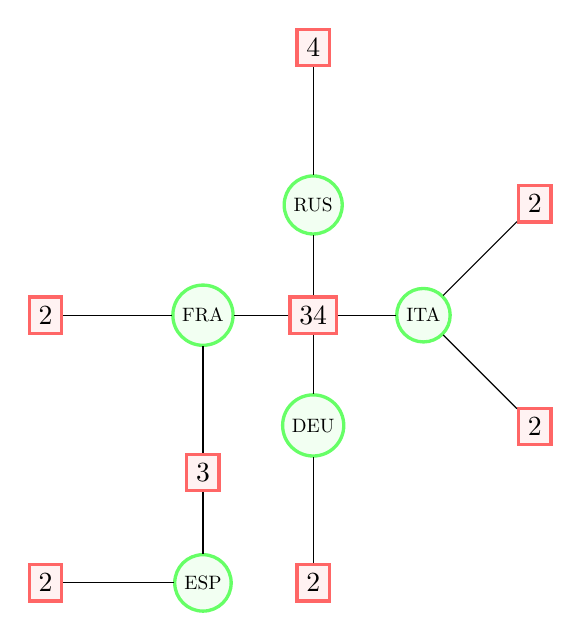
\begin{tikzpicture}[
node distance={20mm},
cutnode/.style={circle, draw=green!60,fill=green!5, very thick, scale=0.7},
blocknode/.style={rectangle, draw=red!60, fill=red!5, very thick}
]
\node[blocknode] (1) {34};
\node[cutnode] (RUS) [above of=1] {RUS};
\node[blocknode] (2) [above of=RUS] {4};
\node[cutnode] (ITA) [right of=1] {ITA};
\node[blocknode] (3) [above right of=ITA] {2};
\node[blocknode] (4) [below right of=ITA] {2};
\node[cutnode] (DEU) [below of=1] {DEU};
\node[blocknode] (5) [below of=DEU] {2};
\node[cutnode] (FRA) [left of=1] {FRA};
\node[blocknode] (6) [below of=FRA] {3};
\node[cutnode] (ESP) [below of=6] {ESP};
\node[blocknode] (7) [left of=ESP] {2};
\node[blocknode] (8) [left of=FRA] {2};

\draw (1) -- (RUS);
\draw (RUS) -- (2);

\draw (1) -- (ITA);
\draw (3) -- (ITA);
\draw (4) -- (ITA);

\draw (1) -- (DEU);
\draw (5) -- (DEU);

\draw (1) -- (FRA);
\draw (6) -- (FRA);
\draw (8) -- (FRA);

\draw (6) -- (ESP);
\draw (7) -- (ESP);
\end{tikzpicture}
\caption{Block-cut tree}\label{fig:block-cut-tree}
\end{figure}

The block-cut tree is shown in \cref{fig:block-cut-tree}.

\item \textbf{Find all edge-biconnected components of \(\EGraph\)}.
The algorithm is similar to finding all biconnected components, except we're
now looking for bridges, not cut-vertices.
\href{https://github.com/ablearthy-itmo-39828cf299f04949c86/discrete-math-2-hw-1/blob/1a4ed14/data/edge_biconnected_components.txt}{Raw data}
obtained by
\href{https://github.com/ablearthy-itmo-39828cf299f04949c86/discrete-math-2-hw-1/blob/7121231/auto/edges_biconnected_components.py}{a script}.

\begin{enumerate}
\item \texttt{PRT}
\item \texttt{SMR}
\item \texttt{VAT}
\item \texttt{MCO}
\item \texttt{DNK}
\item \texttt{ARM},\texttt{ALB},\texttt{AND},\texttt{AUT},\texttt{BLR},
      \texttt{BEL},\texttt{BIH},\texttt{BGR},\texttt{HRV},\texttt{CZE},
      \texttt{EST},\texttt{FIN},\texttt{FRA},\texttt{DEU},\texttt{GEO},
      \texttt{GRC},\texttt{HUN},\texttt{ITA},\texttt{ROK},\texttt{LVA},
      \texttt{LIE},\texttt{LTU},\texttt{LUX},\texttt{MDA},\texttt{MNE},
      \texttt{NLD},\texttt{MKD},\texttt{NOR},\texttt{POL},\texttt{ROU},
      \texttt{RUS},\texttt{SRB},\texttt{SVK},\texttt{SVN},\texttt{ESP},
      \texttt{SWE},\texttt{CHE},\texttt{TUR},\texttt{UKR}
\item \texttt{CYP}
\item \texttt{ISL}
\item \texttt{GBR}
\item \texttt{IRL}
\item \texttt{MLT}
\end{enumerate}

\item Let's define weight function \(w : E \to \mathbb{R}\).

How to calculate distance between two points on the Earth with given coordinates \(\lambda_1, \varphi_1\) and \(\lambda_2, \varphi_2\)?

Let's assume \(R = 6371000\) m. Then
\begin{align*}
x_1 &= R\cos\lambda_1\sin\varphi_1 \\
y_1 &= R\cos\lambda_1\cos\varphi_1 \\
z_1 &= R\sin\lambda_1 \\
x_2 &= R\cos\lambda_2\sin\varphi_2 \\
y_2 &= R\cos\lambda_2\cos\varphi_2 \\
z_2 &= R\sin\lambda_2
\end{align*}

Then,
\[(x_2 - x_1)^2 + (y_2 - y_1)^2 + (z_2 - z_1)^2 = 2 R^2 (1 - \cos\alpha)\]
\[l = 2 \pi R \frac{\alpha}{2 \pi} = R \alpha\]
\begin{align*}
R^2 (\cos\lambda_2\sin\varphi_2 - \cos\lambda_1\sin\varphi_1)^2 &+ \\
R^2 (\cos\lambda_2\cos\varphi_2 - \cos\lambda_1\cos\varphi_1)^2 &+ \\
R^2 (\sin\lambda_2 - \sin\lambda_1)^2 &= 2 R^2 (1 - \cos\alpha) \\
(\cos\lambda_2\sin\varphi_2 - \cos\lambda_1\sin\varphi_1)^2 &+ \\
(\cos\lambda_2\cos\varphi_2 - \cos\lambda_1\cos\varphi_1)^2 &+ \\
(\sin\lambda_2 - \sin\lambda_1)^2 &= 2 (1 - \cos\alpha)
\end{align*}
\begin{align*}
\cos^2\lambda_2\sin^2\varphi_2 - 2\cos\lambda_2\cos\lambda_1\sin\varphi_2\sin\varphi_1 + \cos^2\lambda_1\sin^2\varphi_1 &+ \\
\cos^2\lambda_2\cos^2\varphi_2 - 2\cos\lambda_2\cos\lambda_1\cos\varphi_2\cos\varphi_1 + \cos^2\lambda_1\cos^2\varphi_1 &+ \\
\sin^2\lambda_2 - 2\sin\lambda_2\sin\lambda_1 + \sin^2\lambda_1 &= 2 (1 - \cos\alpha) \\
2 (1 - \cos\lambda_1\cos\lambda_2\cos\delta\varphi + \sin\lambda_1\sin\lambda_2) &= 2 (1 - \cos\alpha)
\end{align*}
\begin{align*}
\alpha = \arccos(\cos\lambda_1\cos\lambda_2\cos\delta\varphi + \sin\lambda_1\sin\lambda_2) \\
l = R\alpha = R\arccos(\cos\lambda_1\cos\lambda_2\cos\delta\varphi + \sin\lambda_1\sin\lambda_2)
\end{align*}

Calculation of distances can be found
\href{https://github.com/ablearthy-itmo-39828cf299f04949c86/discrete-math-2-hw-1/blob/832da1b/auto/mygraph/distances.py}{here}.

In order to build MST I use Prim's algorithm \cite{algoprim} (\href{https://github.com/ablearthy-itmo-39828cf299f04949c86/discrete-math-2-hw-1/blob/5337ff8/auto/mst.py}{script}).

The \textbf{answer} is \(14994452.24596812\) m.

\item \textbf{Find \(\centroid(T)\)}.
Calculate maximum weight of subtree for each vertex and then find minimum
(\href{https://github.com/ablearthy-itmo-39828cf299f04949c86/discrete-math-2-hw-1/blob/53131e2/auto/centroid.py}{script}).

The \textbf{answer} is \textbf{MKD}.

\item \textbf{Construct the Pr\"ufer code for \(T\)}.

The tree is labeled with country code (three letters). Labels are compared lexicographically.
On each iteration remove the lowest leaf from tree, and write its neighbour label.
My
\href{https://github.com/ablearthy-itmo-39828cf299f04949c86/discrete-math-2-hw-1/blob/b4044c9/auto/prufer_code.py}{implementation}
is inefficient, however, for know, it's enough.

\texttt{DEU} \texttt{CZE} \texttt{AUT} \texttt{LVA} \texttt{ARM} \texttt{TUR} \texttt{SVK} \texttt{BEL} \texttt{LTU} \texttt{FRA} \texttt{BEL} \texttt{FRA} \texttt{SWE} \texttt{LTU} \texttt{BLR} \texttt{ESP} \texttt{AND} \texttt{FRA} \texttt{CHE} \texttt{LIE} \texttt{AUT} \texttt{MKD} \texttt{ITA} \texttt{BIH} \texttt{AUT} \texttt{SVN} \texttt{FIN} \texttt{RUS} \texttt{BLR} \texttt{UKR} \texttt{GRC} \texttt{MKD} \texttt{MDA} \texttt{ROU} \texttt{BGR} \texttt{MKD} \texttt{ALB} \texttt{MNE} \texttt{BIH} \texttt{HRV} \texttt{SVN} \texttt{ITA}
\end{enumerate}

\problem Prove

\begin{theorem}[Triangle Inequality]
For any connected graph \(G = \langle V, E \rangle\):
\[\forall x,y,z \in V : \dist(x, y) + \dist(y, z) \ge \dist(x, z)\]
\end{theorem}

\begin{proof}
Assume it's wrong.
\[\exists x,y,z \in V : \dist(x, y) + \dist(y, z) < \dist(x, z)\]
Since \(\dist(x, z)\) is the shortest path, then, according to the assumption,
the shortest path is the path that visits \(y\), so \(\dist(x, z) = \dist(x, y) + \dist(y, z)\).
However, it contradicts our assumption. Therefore,
\[\forall x,y,z \in V : \dist(x, y) + \dist(y, z) \ge \dist(x, z)\]
is true.
\end{proof}

\begin{theorem}[Tree]
A connected graph \(G = \langle V, E \rangle\) is a tree \textit{iff} \(|E| = |V| - 1\)
\end{theorem}

\begin{proof}
Assume \(G\) is a tree. Let's proof that it implies \(|E| = |V| - 1\) by
induction. Base case: \(|V| = 1\), no edges, therefore \(0 = 1 - 1 = 0\). Step:
\(|E| = |V| - 1\). Now add one more vertex. We can add only one edge, otherwise
\(G\) is either a forest or a graph that contains cycle (since at least two
vertices are connected with a new one, it's possible to find a closed walk). So
\(|E| + 1 = |V| - 1 + 1\), therefore \(|E| = |V| - 1\).

Let's prove the following statement: if \(G\) has cycle or more than one
  connected component, then either \(|E| > |V| - 1\) or \(|E| < |V| - 1\).
The \(|E| < |V| - 1\) case is possible if there are more than one connected components.
Now let's talk about \(|E| > |V| - 1\) case. Since we're working with discrete values, then \(|E| > |V| - 1 \iff |E| \ge |V|\).
Let's focus on the cycle. It's obvious that in the cycle the following is true \(|E| \ge |V|\).
Adding a vertex that is in another connected component will increase \(|V|\), so \(|E| \ge |V| + 1\) (forest).
Otherwise adding a vertex will increase both \(|E|\) and \(|V|\), so \(|E| + m \ge |V| + 1 \implies |E| \ge |V|\).

By contraposition, if \(|E| = |V| - 1\), then \(G\) has no cycles and has only one connected component (i.e. it's a tree).
\end{proof}

\begin{theorem}[Hall]
For any bipartite graph \(G = (X, Y, E)\), there exists \(X\)-perfect matching
\textit{iff} \(|N(W)| \ge |W|\) for every \(W \subseteq X\).
\end{theorem}

\begin{proof}
Let \(M\) be a \(X\)-perfect matching.
The "only if" part: For every \(x \in W\) there's \(y \in Y\) such that \(xy \in M\).
Therefore, the amount of number is at least \(|W|\).

The "if" part. Let's prove contraposition.
Assume there's no \(X\)-perfect matching.
Therefore, for each matching \(M : |M| < |X|\).
Let \(U\) be a minimum vertex cover and \(U_x = U \cap X\), \(U_y = U \cap Y\).
According to K\"onig's theorem, the number of edges in maximal matching equals
the number of vertices in minimum vertex cover.
Therefore, \(|U| = |M| < |X|\). Therefore, \(|U_x| + |U_y| = |U| < |X|\).

Let \(W = X \setminus U_x\). \(|W| = |X| - |U_x|\).
The neighbours of \(W\) are elements from \(U_y\).
Otherwise \(U\) is not minimum vertex cover:
if \(\exists y \in Y : y \not\in U_y \land y \in N(W)\),
then there's uncovered edge, therefore \(U\) is not vertex cover, contradiction.
Therefore, \(N(W) = U_y\), therefore \(|N(W)| = |U_y| = |U| - |U_x|\).
\[|N(w)| = |U_y| < |X| - |U_x| = |W|\]
Therefore, \(|N(w)| < |W|\). Contraposition is proved, therefore
the original statement is proved too.
\end{proof}

\begin{theorem}[Whitney]
For any graph \(G\): \(\varkappa(G) \le \lambda(G) \le \delta(G)\)
\end{theorem}

\begin{proof}
The \(\varkappa(G) \le \lambda(G)\) part:
assume \(\varkappa(G) > \lambda(G)\).
However, let \(P\) be a set of edges removal of which makes \(G\) disconnected.
Therefore, \(|P| = \lambda(G)\).
In the worst case we can remove \(|P|\) vertices that are incident with edges
from \(P\). So, in the worst case \(\varkappa(G) = \lambda(G)\).
However, it's possible to remove less than \(\lambda(G)\) vertices, therefore
\(\varkappa(G) > \lambda(G)\) is wrong.

The \(\lambda(G) \le \delta(G)\) part:
assume \(\lambda(G) > \delta(G)\).
However, removal of all edges that are incident to a vertex with degree
\(\delta(G)\) makes \(G\) disconnected,
therefore at least \(\lambda(G) = \delta(G)\)
(also \(\lambda(G)\) can be less than \(\delta(G)\)).
Contradiction. The assumption was wrong, so \(\lambda(G) \le \delta(G)\) holds.
\end{proof}

\begin{theorem}[Chartrand]
For a connected graph \(G = \langle V, E \rangle\)
\[\delta(G) \ge \lfloor \frac{|V|}{2} \rfloor \implies \lambda(G) = \delta(G)\]
\end{theorem}

\begin{proof}
According to a previous theorem \(\lambda(G) \le \delta(G)\).
We can show that \(\lambda(G) < \delta(G)\) doesn't hold.

Removal of \(\lambda(G)\) edges makes it disconnected, so we can divide
vertices into two sets \(A\) and \(V \setminus A\) that can be connected via
\(\lambda(G)\) edges.

Let \(P\) be a minimum set of edges that can be removed to make \(G\) disconnected.
\(|P| = \lambda(G)\)

Assume \(m\) vertices from \(A\) are incident to edges from \(P\).
Obviously, \(m \le \lambda(G)\).
If \(|A| = m\), then
The number of edges in \(G\) incident with two vertices of \(A\) is at least
\(\frac12 (m \delta(G) - \lambda(G))\) (from each \(m\) vertex there's at least
\(\delta(G)\) edges minus whose, that connect \(A\) with \(V \setminus A\);
since we encountered each edge twice, divide it by 2).
\textit{\textrussian{Заметим, что}}
\(\frac12 (m \delta(G) - \lambda(G)) > \frac12 m (m - 1) = C_{2}^{m}\).
Contradiction, since maximum number of edges is \(C_{2}^{m}\).

If \(|V \setminus A| = m\), then just "swap" \(A\) and \(V \setminus A\).

If \(A\) and \(V \setminus A\) contain vertices adjacent only to vertices in their own subsets, then each subset should contain at least \(\delta(G) + 1\) vertices (to maintain \(\delta(G) \ge \lfloor \frac{|V|}{2}\rfloor\)).
Since \(\delta(G) + 1 \ge \lfloor \frac{|V|}{2} \rfloor + 1\),
then \(2 (\delta(G) + 1) \ge 2 \lfloor \frac{|V|}{2} \rfloor + 2\).
If \(|V|\) is even, then \(2 (\delta(G) + 1) \ge |V| + 2\), contradiction.
IF \(|V|\) is odd, then \(2 (\delta(G) + 1) \ge |V| - 1 + 2 = |V| + 1\), contradiction.

So, assumption \(\lambda(G) < \delta(G)\) is wrong, therefore, \(\lambda(G) =
\delta(G)\).
\end{proof}


\begin{landscape}
\begin{figure}
\centering
\includestandalone[mode=build,width=0.95\linewidth]{maps/basic}
\caption{Basic map}\label{fig:map_basic}
\end{figure}
\end{landscape}

\begin{landscape}
\begin{figure}
\centering
\includestandalone[mode=build,width=0.95\linewidth]{maps/vertex_coloring}
\caption{Vertex coloring}\label{fig:vertex_coloring_map}
\end{figure}
\end{landscape}

\begin{landscape}
\begin{figure}
\centering
\includestandalone[mode=build,width=0.95\linewidth]{maps/edge_coloring}
\caption{Edge coloring}\label{fig:edge_coloring_map}
\end{figure}
\end{landscape}

\begin{landscape}
\begin{figure}
\centering
\includestandalone[mode=build,width=0.95\linewidth]{maps/stable_set}
\caption{Maximum stable set}\label{fig:stable_set_map}
\end{figure}
\end{landscape}

\begin{landscape}
\begin{figure}
\centering
\includestandalone[mode=build,width=0.95\linewidth]{maps/matching}
\caption{Maximum matching}\label{fig:matching_map}
\end{figure}
\end{landscape}

\begin{landscape}
\begin{figure}
\centering
\includestandalone[mode=build,width=0.95\linewidth]{maps/vertex_cover}
\caption{Minimum vertex cover}\label{fig:vertex_cover_map}
\end{figure}
\end{landscape}

\begin{landscape}
\begin{figure}
\centering
\includestandalone[mode=build,width=0.95\linewidth]{maps/edge_cover}
\caption{Minimum edge cover}\label{fig:edge_cover_map}
\end{figure}
\end{landscape}

\printbibliography

\end{document}
